\documentclass[a4paper,12pt]{article}

% Packages
\usepackage{graphicx}
\usepackage{amsmath}
\usepackage{amsfonts}
\usepackage{geometry}
\usepackage{fancyhdr}
\usepackage{setspace}
\usepackage{titlesec}
\usepackage{hyperref}
\usepackage{xcolor}
\usepackage{minted}
\usepackage{dirtytalk}
\usepackage{enumitem}

\setminted[cmake]{
    linenos=false,
    breaklines=true,
    encoding=utf8,
    fontsize=\footnotesize,
    frame=lines
}

\hypersetup{
    colorlinks=true,
    linkcolor=darkgray,
}

\usepackage{etoolbox}
\AtBeginEnvironment{minted}{\dontdofcolorbox}
\def\dontdofcolorbox{\renewcommand\fcolorbox[4][]{##4}}

% Text
\geometry{margin=1in}
\setstretch{1.1}
\setlength{\parskip}{0.8em}
\setlength{\parindent}{1em}
\setlist[itemize]{topsep=-6pt, partopsep=0pt, parsep=0pt, itemsep=0pt}

% Header and Footer
\setlength{\headheight}{14.5pt}
\addtolength{\topmargin}{-2.5pt}
\pagestyle{fancy}
\fancyhf{}
\fancyhead[L]{Jocs per Computador}
\fancyhead[R]{\thepage}

% Image path
\graphicspath{{figs/}}

% Title Formatting
\titleformat{\section}{\normalfont\Large\bfseries}{\thesection}{1em}{}

% Cover Page
\title{
    \vspace{2cm}
    
\includegraphics[width=0.75\textwidth]{fib.png} \\
    \vspace{1cm}
    \textbf{\Huge Jocs per Computador} \\
    \vspace{1cm}
    \large JC-MEI \\
    \vspace{0.5cm}
    \large \today
}
\author{
Carles Matoses Gimenez\\
\small carles.matoses@estudiantat.upc.edu
}
\date{}

\begin{document}

\maketitle
\thispagestyle{empty}
\newpage

\setcounter{page}{1}
\tableofcontents
\newpage

\section{Introducció}
Aquest document descriu el desenvolupament d'un videojoc 2D creat com a part de l'assignatura “Jocs per Computador”. A continuació es detallen els objectius, el disseny, les mecàniques i els reptes implementats durant el projecte.

\section{Objectius}
L'objectiu principal és guiar el jugador a través de diferents pantalles (nivells), on ha d'aconseguir claus, equipar objectes i resoldre trencaclosques per accedir a l'enfrontament final amb el cap de nivell. El mapa del joc es mostra a la figura \ref{fig:mapa}. El jugador comença a l'"overworld" i ha d'accedir a la "dungeon1". Les possibles rutes es mostren en roig; altres colors indiquen dependències entre nivells.

\begin{figure}[ht!]
    \centering
    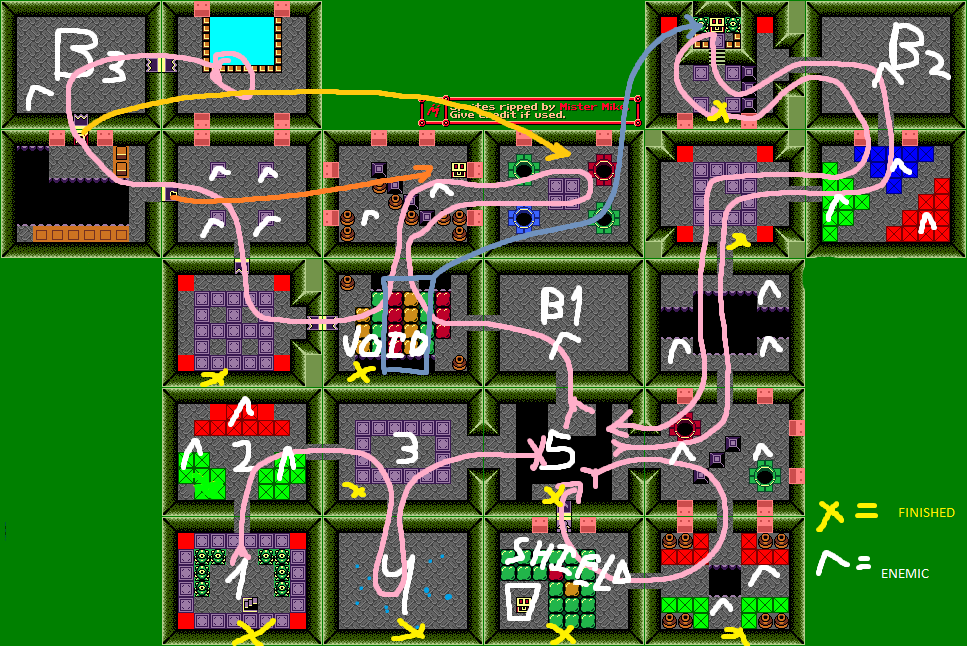
\includegraphics[width=0.8\textwidth]{../imgs/recorregut.png}
    \caption{Mapa del joc amb el recorregut i els requisits per a cada nivell.}
    \label{fig:mapa}
\end{figure}

\section{Disseny del Joc}

\subsection{Arquitectura General}
No s'ha seguit un patró concret, però s'ha utilitzat una classe auxiliar anomenada \textbf{GameStateManager} per gestionar els estats del joc. Aquesta estructura permet afegir o eliminar estats dinàmicament. Els estats són independents i poden rebre inputs, fer actualitzacions i pintar en pantalla.

\subsection{Gestió de Col·lisions}
Els objectes del joc tenen una "bounding box" i es comprova el solapament entre elles per detectar col·lisions. Aquestes poden ser:
\begin{itemize}
    \item \textbf{onCollide(item)}: quan dos objectes col·lisionen.
    \item \textbf{SteppedOn}: per saber si el jugador està damunt d'un cert objecte.
\end{itemize}
Els atacs també generen una bounding box temporal per detectar col·lisions amb enemics o objectes.

\subsection{Nivells i Escenes}
La jerarquia del joc consisteix en:
\begin{itemize}
    \item \texttt{World}: conté un diccionari de mapes.
    \item \texttt{Mapa}: llista de nivells.
    \item \texttt{Level}: llista d'elements i entitats.
\end{itemize}
\texttt{Scene} actualitza els nivells i interactua amb una còpia local dels elements. En sortir d'un nivell, aquest es reinicia a l'estat original per defecte.

\begin{figure}[ht!]
    \centering
    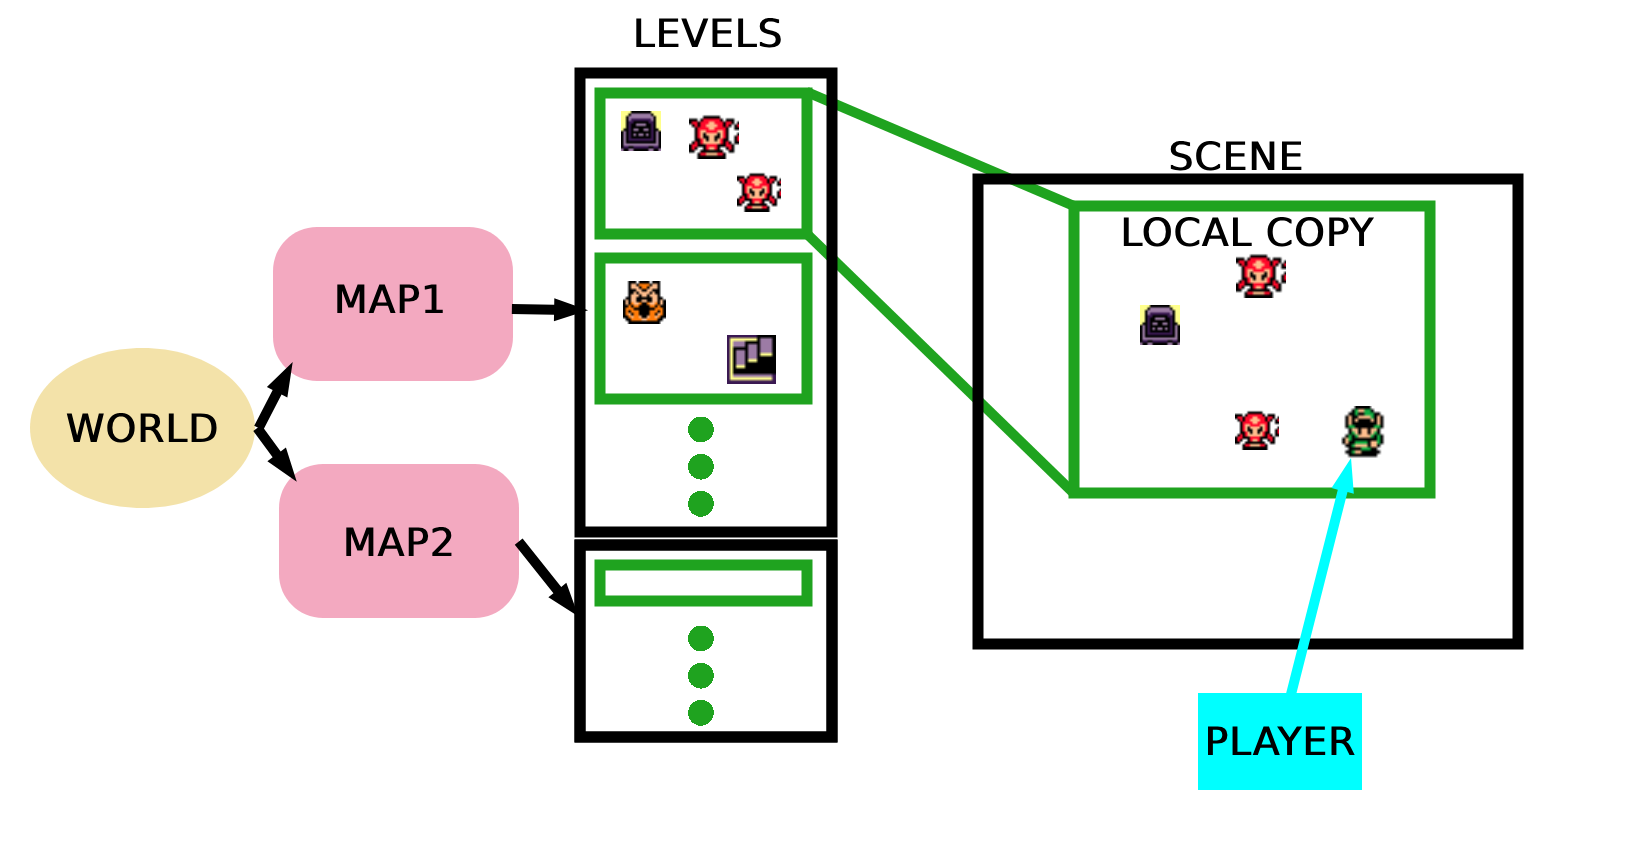
\includegraphics[width=0.8\textwidth]{../imgs/global_to_local.png}
    \caption{Jerarquia dels elements durant l'execució del joc.}
    \label{fig:global_to_local}
\end{figure}

\subsubsection{Categories d'elements i entitats}
\begin{itemize}
    \item \textbf{Items equipables}: Espasa, Escut, Ploma, Braçalet
    \item \textbf{Items}: Claus
    \item \textbf{Blocs decoratius}: Portcullis, Lights, Vase, Fire Place, Animated Floor
    \item \textbf{Blocs interactius}: Làpides, Cofres, Rotors, Portes, Estatues, Floating Heart/Money
    \item \textbf{Entitats}: Jugador, Enemics, Bosses, NPCs
\end{itemize}

\section{Mecàniques de Joc}

\subsection{Equipar Items}
Els items es poden equipar a través de l'inventari. Proporcionen habilitats (força, volar, etc.).

\subsection{Combat}
El jugador pot atacar amb la seva arma i interactuar amb certs objectes destructibles.

\subsection{Interacció}
Amb la tecla principal, el jugador pot obrir cofres, parlar amb NPCs, activar portes, etc.

\subsection{Triggers}
\textbf{Triggers} disponibles:
\begin{itemize}
    \item \texttt{onEnter}, \texttt{onExit}, \texttt{onAllEnemiesDead}
    \item Triggers personalitzats per modificar elements específics (ex: làpida de la cova de la mort)
\end{itemize}

\section{Trencaclosques Implementats}

\subsection{Lights Out}
Un trencaclosques basat en el clàssic joc de taula. Es resol apagant totes les llums d'una graella interactiva.

\begin{figure}[ht!]
    \centering
    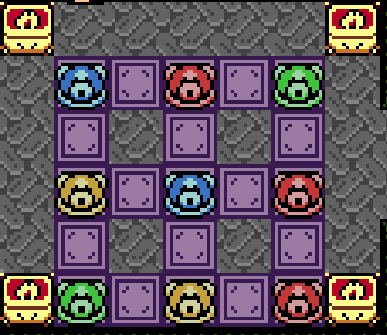
\includegraphics[width=0.6\textwidth]{../imgs/exemple-trencaclosques.png}
    \caption{Exemple del trencaclosques "Lights Out" implementat.}
    \label{fig:exemple-trencaclosques}
\end{figure}

\subsection{Objectes Pesats}
Alguns objectes (com làpides o pedres) es poden empènyer amb un item específic (Braçalet) que proporciona força. Exemples:
\begin{itemize}
    \item Làpida de la cova de la mort (obri pas a la "dungeon1")
    \item Pedres que bloquegen l'accés a la "Feather"
\end{itemize}

\subsection{Preguntes i Respostes}
Algunes estàtues requereixen una resposta correcta per activar triggers especials.

\section{Enemics}
S'han implementat enemics comuns com slimes, ratpenats, etc. També s'inclouen caps amb comportaments personalitzats. Els enemics poden morir, i això pot desbloquejar portes o activar triggers.

\section{Menús i Interfície}

\begin{itemize}
    \item \textbf{Start}: Menú inicial per començar o eixir del joc
    \item \textbf{In-Game Menu}: Accés durant el joc mitjançant ESC
    \item \textbf{Controls}: Llista de controls
    \item \textbf{Credits}: Crèdits del projecte
    \item \textbf{Final Menu}: Menú especial al completar el joc
    \item \textbf{Diàlegs}: Sistema de diàlegs amb NPCs, amb múltiples opcions
\end{itemize}

\section{Limitacions i Consideracions}

\subsection{Gestió de la mort}
La mort del jugador no està implementada de forma completa. Si el jugador mor, apareix en una pantalla anterior com si no hagués passat res. Això pot causar problemes amb triggers, especialment amb bosses que esperen només una execució inicial.

Solució provisional: afegir múltiples comprovacions per assegurar que l'estat del boss es manté coherent.

\end{document}
